

Pour la réalisation d'une simulation sur des robots, nous avons du implémenter un architecture afin de permettre à nos programme de gérer d'une part nos robots et d'autre part de voir si le résultat théorique correspond aux résultats expérimentaux.

\medskip

Nous aboutissons au final à l'architecture suivante:

\bigskip

\begin{figure}[ht]
\centering
    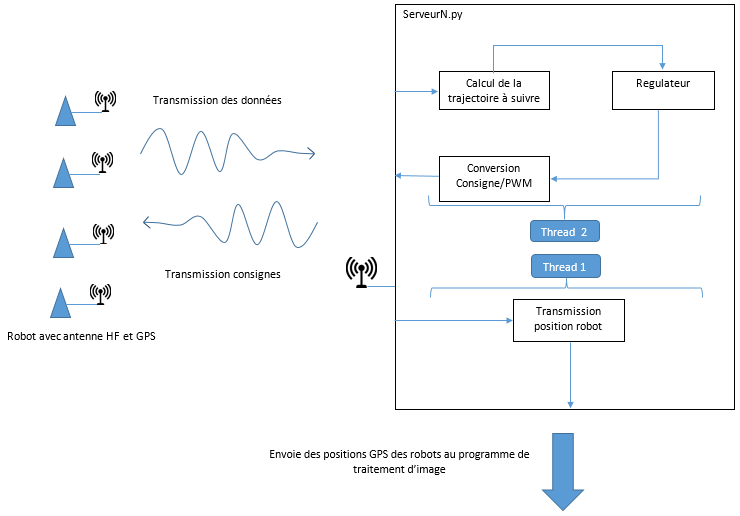
\includegraphics[scale=0.8,angle=0]{SyntheseExp.PNG}
    \caption{Architecture mise en place pour la simulation sur robot char.}
    \label{fig:SyntheseExp}
\end{figure}

\bigskip
\subsection{GPS}
ici la description des GPS utilisés
\subsection{Robot}
ici la description des robots et des récepteurs
